\section{Definirea problemei}
% enuntul intrebarii
În această secțiune vom prezenta problma fiecărui puzzle.
\newline


\subsection{AllOut - 4x4}

\newline\newline
 \newline \newline Ne este dată o matrice de 4 coloane și 4 rânduri, în care unele dintre celule sunt luminate. Scopul este de a stinge toate celulele prin selectarea celulelor în ordine corectă. Când o celulă este selectată, cele din jurul ei(vecinii) se vor schimba din starea lor curentă. Jucătorul trebuie să folosească această caracteristică pentru a stinge toate celulele în cel mai scurt timp posibil și cu cele mai puține mișcări posibile.\newline
\newline Am creat 2 astfel de lvl pentru a le compara timpul de execuție.\newline
 \newline
  \newline
\begin{figure}[h]
\centering
 
\includegraphics[width=0.4\textwidth]{text/images/pic2.jpeg}\
  \hfill
  
\includegraphics[width=0.4\textwidth]{text/images/pic3.jpeg}\
   \newline
    \caption{AllOut 4x4}
\end{figure} \newline \newline
 \newline După cum se observă și în poze, avem 2 situații cu câte 5 lumini aprinse, iar restul sunt stinse.
Se poate găsi o posibilitate pentru a stinge toate luminile?
Vom afla la implementare.

\pagebreak
\subsection{AllOut - 5x5}

\newline
Ne este dată o matrice de 5 coloane și 5 rânduri. Acest lvl este mai greu de implementat și de rezolvat. Implicit timpul va fi mai mare, de aceea ne trebuie o strategie cât mai bună.\newline \newline
  \newline
  \newline
\begin{figure}[h]
\centering
 
\includegraphics[width=0.4\textwidth]{text/images/pic4.jpeg}\
  \hfill
  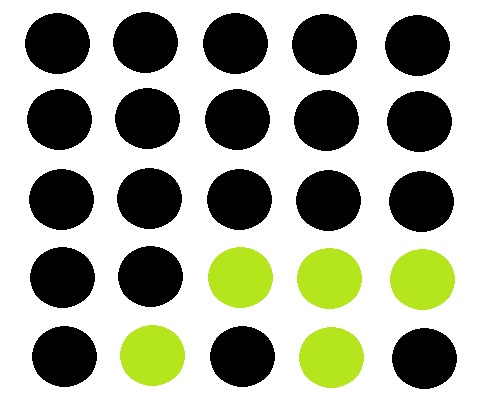
\includegraphics[width=0.4\textwidth]{text/images/pic5.jpeg}\
   \newline
    \caption{AllOut 5x5}
\end{figure} \newline \newline
\newline

\newline \newline După cum se observă și în poze, avem 2 situații: prima cu 10 lumini aprinse, iar cealaltă cu 5 lumini aprinse. \newline\newline
Diferența principală dintre un puzzle "Allout" de dimensiune 4x4 și unul de dimensiune 5x5 este mărimea grid-ului și numărul de celule care trebuie stinse. Într-un puzzle de dimensiune 4x4, există 16 celule în total, în timp ce într-un puzzle de dimensiune 5x5 există 25 de celule. \newline\newline
Acest lucru înseamnă că un puzzle de dimensiune 5x5 va fi mai dificil de rezolvat și va necesita mai multă gândire strategică din partea jucătorului. De asemenea, un puzzle de dimensiune 5x5 poate include celule suplimentare care au reguli speciale sau comportamente care îl fac mai complex și mai dificil de rezolvat decât 4x4.

\pagebreak